\documentclass[10pt,openright,twoside,french]{book}

\input philippe2013
\input philippe2013_cours
\input philippe2013_sections
\input philippe2013_chapitre
\renewcommand\PartProgramme{Analyse}
\renewcommand\MaCouleur{Purple}

\pieddepage{}{%
\begin{tikzpicture}[scale=0.65]
\shadedraw [top color=white, bottom color=\MaCouleur, draw=\MaCouleur]
[l-system={Sierpinski triangle, step=1pt, angle=60, axiom=F, order=6.5}]
lindenmayer system -- cycle;
\draw (30:0.65cm) node {\bfseries\textcolor{black}{\thepage}};
\end{tikzpicture}%
}{}

\setcounter{chapter}{2}
\begin{document}
\chapter{Cercle trigonométrique}\label{cercle_trigo}

\section{Angles dans un cercle}
\begin{Defi}
    Un \ipt{angle} est une surface délimitée par deux demies-droites (les \iptb{côtés} de l'angle) de même origine appelée \iptb{sommet} de l'angle.\par
    Le \ipt{degré} est une unité de mesure permettant de mesurer l'écart entre les deux demi-droites, appelé \iptb{mesure} de l'angle.
\end{Defi}

\begin{Rmq}
    On s'intéressera dans ce cours à l'angle saillant.
    \begin{center}
    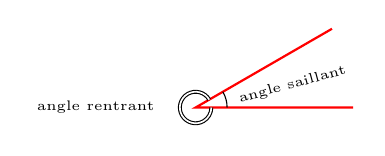
\begin{tikzpicture}
        % angle de 30°
        \pgfmathparse{2*cos(30)}\let\x\pgfmathresult
        \pgfmathparse{2*sin(30)}\let\y\pgfmathresult
        \draw[red,thick] (2,0) -- (0,0) -- (\x,\y);
        \draw[thin] (.4,0) arc (0:30:.4cm);
        \node[right] at (35:.5) {\tiny \rotatebox{15}{angle saillant}};
        %
        \draw[double,thin] (30:0.2) arc (30:360:.2cm);
        \node[left] at (180:.4) {\tiny angle rentrant};
    \end{tikzpicture}
    \end{center}
\end{Rmq}

\subsection{Cercle trigonométrique}

\begin{Defi}
    On considère un repère orthonormé $(O,I,J)$ du plan.\par
    On appelle \ipt{cercle trigonométrique} le cercle $\calig U$ de centre $O$ et de rayon $1$.
\end{Defi}

\begin{Rmq}
    On s'intéressera dans ce cours à un point $M$ situé sur $\calig U$ et à l'angle $\widehat{IOM}$ formé par les demies-droites $[OI)$ et $[OM)$ ainsi qu'à sa mesure $\theta$.
    \begin{center}
    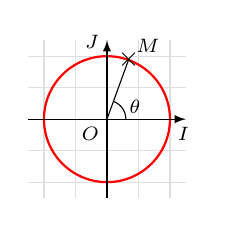
\begin{tikzpicture}[scale = 0.4]
        \draw[thin, color=gray!25] (-2.5,-2.5) grid (2.5,2.5);
        \draw[red,thick] (0,0) circle (2cm);
        \draw[->,>=latex] (-2.5,0)--(2.5,0);
        \draw[->,>=latex] (0,-2.5)--(0,2.5);
        \coordinate (O) at (0,0);
        \coordinate (I) at (2,0);
        \coordinate (J) at (0,2);
        \coordinate (M) at (70:2cm);
        \draw (M) node {$\times$};
        \begin{scriptsize}
            \draw (O) node[below left]{$O$};
            \draw (I) node[below right]{$I$};
            \draw (J) node[above left]{$J$};
            \draw (M) node [above right] {$M$};
            \draw (O) -- (M);
            \draw (0.6,0) arc (0:70:0.6cm);
            \draw (40:0.6cm) node[right] {$\theta$};
        \end{scriptsize}
    \end{tikzpicture}
    \end{center}
\end{Rmq}

\begin{Defi}
    Dans le cercle trigométrique, on appelle \ipt{sens trigonométrique}, ou sens direct, le sens qui parcourt le cercle dans le sens inverse des aiguilles d'une montre.\par
    Dans le sens trigonométrique, la mesure d'un angle sera positive ; dans le sens indirect, la mesure sera négative.
    \begin{center}
    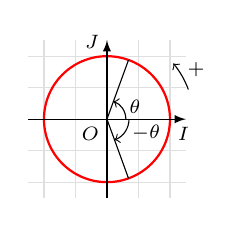
\begin{tikzpicture}[scale = 0.4]
        \draw[thin, color=gray!25] (-2.5,-2.5) grid (2.5,2.5);
        \draw[red,thick] (0,0) circle (2cm);
        \draw[->,>=latex] (-2.5,0)--(2.5,0);
        \draw[->,>=latex] (0,-2.5)--(0,2.5);
        \coordinate (O) at (0,0);
        \coordinate (I) at (2,0);
        \coordinate (J) at (0,2);
        \coordinate (M) at (70:2cm); \draw (O) -- (M);
        \coordinate (N) at (-70:2cm); \draw (O) -- (N);
        \draw[->] (20:2.75cm) arc (20:40:2.75cm);
        \draw (35:2.75cm) node[right] {\scriptsize $+$};
        \begin{scriptsize}
            \draw (O) node[below left]{$O$};
            \draw (I) node[below right]{$I$};
            \draw (J) node[above left]{$J$};
            \draw[->] (0.6,0) arc (0:70:0.6cm);
            \draw (40:0.6cm) node[right] {$\theta$};
            \draw[->] (0.7,0) arc (0:-70:0.7cm);
            \draw (-40:0.7cm) node[right] {$-\theta$};
        \end{scriptsize}
    \end{tikzpicture}
    \end{center}
\end{Defi}

\subsection{Mesurer un angle en radian}

\begin{Defi}
    On considère le cercle trigonométrique $\calig U$ ainsi qu'un point $M$ sur ce cercle.\par
    La mesure de l'angle $\widehat{IOM}$, exprimée en \ipt{radian}, est égale à la longueur de l'arc $\Arc{IM}$ dans le sens trigonométrique et est égale à l'opposé de la longueur de l'arc $\Arc{IM}$ dans le sens indirect.

\begin{center}
    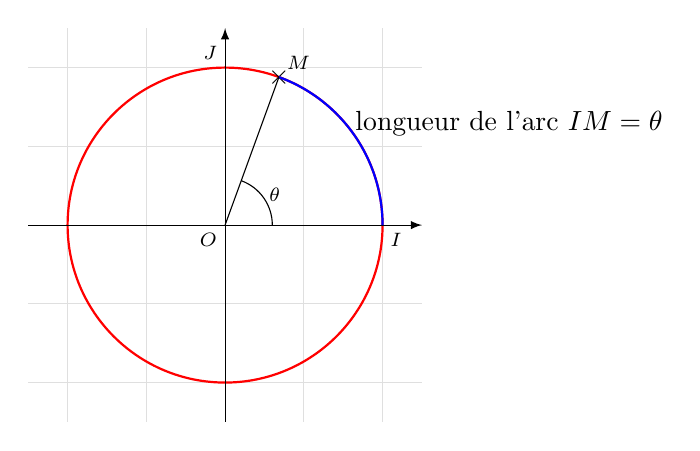
\begin{tikzpicture}
        \draw[thin, color=gray!25] (-2.5,-2.5) grid (2.5,2.5);
        \draw[red,thick] (0,0) circle (2cm);
        \draw[->,>=latex] (-2.5,0)--(2.5,0);
        \draw[->,>=latex] (0,-2.5)--(0,2.5);
        \coordinate (O) at (0,0);
        \coordinate (I) at (2,0);
        \coordinate (J) at (0,2);
        \coordinate (M) at (70:2cm);
        \draw (M) node {$\times$};
        \draw[thick,blue] (2,0) arc (0:70:2cm);
        \draw (40:2cm) node[right] {longueur de l'arc $\Arc{IM} = \theta$};
        \begin{scriptsize}
            \draw (O) node[below left]{$O$};
            \draw (I) node[below right]{$I$};
            \draw (J) node[above left]{$J$};
            \draw (M) node [above right] {$M$};
            \draw (O) -- (M);
            \draw (0.6,0) arc (0:70:0.6cm);
            \draw (40:0.6cm) node[right] {$\theta$};
        \end{scriptsize}
    \end{tikzpicture}
\end{center}
\end{Defi}

\begin{Exemple}[s]
\begin{enumerate}
    \item Lorsque le point $M$ est confondu au point $I$, la longueur de l'arc $\Arc{IM}$ est égal à $0$ donc on obtient $\widehat{IOM} = 0 \text{ rad}$.
    \item Si on suppose maintenant que le point $M$ a effectué un tour complet autour du cercle dans le sens trigonométrique, on trouve que la longueur de l'arc $\Arc{IM}$ est égal au périmètre $\calig P$ du cercle. Or, $\calig P = 2\pi r$ et $r = 1$ donc on obtient $\widehat{IOM} = 2\pi \text{ rad}$.
    \item Si on effectue à présent un quart de tour dans le sens direct, on aura $\widehat{IOM} = \frac{2\pi}{4} = \frac\pi2 \text{ rad}$.
    \item Si on effectue à présent un quart de tour dans le sens indirect, on aura $\widehat{IOM} = -\frac{2\pi}{4} = -\frac\pi2 \text{ rad}$.
\begin{center}
    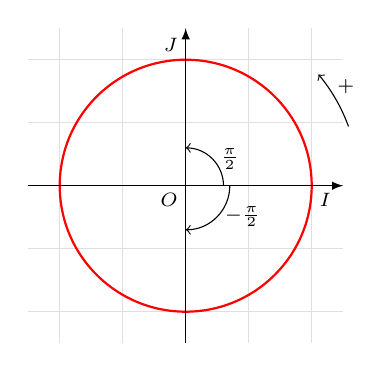
\begin{tikzpicture}[scale=0.8]
        \draw[thin, color=gray!25] (-2.5,-2.5) grid (2.5,2.5);
        \draw[red,thick] (0,0) circle (2cm);
        \draw[->,>=latex] (-2.5,0)--(2.5,0);
        \draw[->,>=latex] (0,-2.5)--(0,2.5);
        \coordinate (O) at (0,0);
        \coordinate (I) at (2,0);
        \coordinate (J) at (0,2);
        \coordinate (M) at (90:2cm); \draw (O) -- (M);
        \coordinate (N) at (-90:2cm); \draw (O) -- (N);
        \draw[->] (20:2.75cm) arc (20:40:2.75cm);
        \draw (35:2.75cm) node[right] {\scriptsize $+$};
        \begin{scriptsize}
            \draw (O) node[below left]{$O$};
            \draw (I) node[below right]{$I$};
            \draw (J) node[above left]{$J$};
            \draw[->] (0.6,0) arc (0:90:0.6cm);
            \draw (45:0.6cm) node[right] {$\frac\pi 2$};
            \draw[->] (0.7,0) arc (0:-90:0.7cm);
            \draw (-45:0.7cm) node[right] {$-\frac\pi 2$};
        \end{scriptsize}
    \end{tikzpicture}
    \end{center}
\end{enumerate}
\end{Exemple}\medskip

L'exemple précédent nous montre qu'une même position pour le point $M$ peut entraîner différentes mesures d'un angle, en fonction du nombre de tours effectués par $M$. Les différentes mesures diffèrent donc d'un multiple de $2\pi$ qui correspond au périmètre du cercle trigonométrique. On a donc :

\begin{Prop}
    On considère un point $M$ sur le cercle $\calig U$.
    \begin{enumerate}
        \item L'angle $\widehat{IOM}$ possède une infinité de mesure.
        \item Pour deux mesures $x$ et $y$, il existe $k \in \Z$ tel que $y = x + 2k\pi$.
        \item Il n'existe qu'une seule mesure dans l'intervalle $\intervalleof{-\pi}{\pi}$.
    \end{enumerate}
\end{Prop} \medskip

Afin de garantir l'unicité de certains résultats, on est amené à définir la notion de mesure principale d'un angle :

\begin{Defi}
    On considère un point $M$ sur le cercle $\calig U$.
    Parmi toutes les mesures de l'angle $\widehat{IOM}$, on appelle \ipt{mesure principale} celle qui appartient à l'intervalle $\intervalleof{-\pi}{\pi}$.
\end{Defi}\clearpage

\begin{Exemple}
    On considère un angle de mesure $\alpha = \frac{43\pi}{4}$. Déterminer la mesure principale de cet angle et placer $M$ sur $\calig U$ tel que $\widehat{IOM} = \alpha$.\par\medskip
    Il suffit de trouver $k \in \Z$ tel que $\frac{43\pi}{4} = x + 2k\pi$ et $x$ sera alors la mesure principale cherchée.\par
    On réduit tout d'abord au même dénominateur : $2\pi = \frac{8\pi}{4}$ puis on effectue la division euclidienne de $43$ par $8$ : $43 =5\times 8 + 3$.\par\medskip
    Ainsi : $\frac{43\pi}{4} = \frac{5 \times 8\pi}{4} + \frac{3\pi}{4} = 5 \times 2\pi + \frac{3\pi}{4}$ donc la mesure principale de l'angle est $\frac{3\pi}{4}$.

\begin{center}
    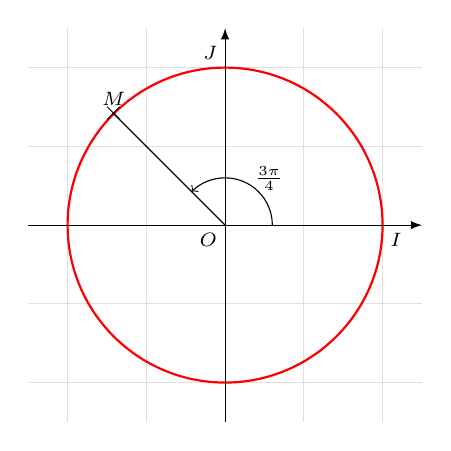
\begin{tikzpicture}
        \draw[thin, color=gray!25] (-2.5,-2.5) grid (2.5,2.5);
        \draw[red,thick] (0,0) circle (2cm);
        \draw[->,>=latex] (-2.5,0)--(2.5,0);
        \draw[->,>=latex] (0,-2.5)--(0,2.5);
        \coordinate (O) at (0,0);
        \coordinate (I) at (2,0);
        \coordinate (J) at (0,2);
        \coordinate (M) at (135:2cm);
        \draw (M) node {$\times$};
        \begin{scriptsize}
            \draw (O) node[below left]{$O$};
            \draw (I) node[below right]{$I$};
            \draw (J) node[above left]{$J$};
            \draw (M) node [above] {$M$};
            \draw (O) -- (M);
            \draw[->] (0.6,0) arc (0:135:0.6cm);
            \draw (80:0.6cm) node[right=5pt] {$\frac{3\pi}{4}$};
        \end{scriptsize}
    \end{tikzpicture}
    \end{center}
\end{Exemple}

\subsection{Quelques conversions à connaître}

\begin{center}
\renewcommand\arraystretch{2.5}
    \begin{tabular}{*{10}{|c}|}
        \hline
            Angles en degré & $0$ & $360$ & $180$ & $30$ & $45$ & $60$ & $90$ & $270$ & $\alpha$ \\
        \hline
            Angles en radian & $0$ & $2\pi$ & $\frac\pi2$ & $\frac{\pi}{6}$ & $\frac\pi4$ & $\frac\pi3$ & $\frac\pi2$ & $\frac{3\pi}{2}$  & $\alpha \times\frac{2\pi}{360}$\\
        \hline
    \end{tabular}
\end{center}

\section{Cosinus et Sinus d'un nombre réel}
\subsection{Lien avec le cercle trigonométrique}

\begin{Prop}
    On considère un point $M$ sur le cercle $\calig U$ et $\alpha$ un nombre réel tel que $\widehat{IOM} = \alpha$. On ne demande pas à $\alpha$ d'être la mesure principale de l'angle $\widehat{IOM}$.\par
    Le nombre \iptb{$\cos(\alpha)$}\index{cosinus d'un nombre réel} est alors égal à l'abscisse du point $M$ et le nombre \iptb{$\sin(\alpha)$}\index{sinus d'un nombre réel} est égal à l'ordonnée du point $M$.

\begin{center}
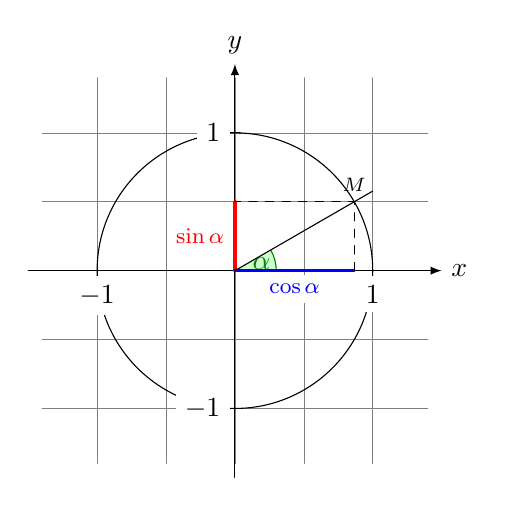
\begin{tikzpicture}[scale=1.75,cap=round]
    % Local definitions
    \def\costhirty{0.8660256}
    % Colors
    \colorlet{anglecolor}{green!50!black}
    \colorlet{sincolor}{red}
    \colorlet{tancolor}{orange!80!black}
    \colorlet{coscolor}{blue}
    % Styles
    \tikzstyle{axes}=[>=latex]
    \tikzstyle{important line}=[very thick]
    \tikzstyle{information text}=[rounded corners,fill=red!10,inner sep=1ex]
    % The graphic
    \draw[style=help lines,step=0.5cm] (-1.4,-1.4) grid (1.4,1.4);
    \draw (0,0) circle (1cm);
    \begin{scope}[style=axes]
        \draw[->] (-1.5,0) -- (1.5,0) node[right] {$x$} coordinate(x axis);
        \draw[->] (0,-1.5) -- (0,1.5) node[above] {$y$} coordinate(y axis);
        \foreach \x in {-1,1} \draw[xshift=\x cm] (0pt,1pt) -- (0pt,-1pt) node[below,fill=white] {$\x$};
        \foreach \y in {-1,1} \draw[yshift=\y cm] (1pt,0pt) -- (-1pt,0pt) node[left,fill=white] {$\y$};
    \end{scope}
    \filldraw[fill=green!20,draw=anglecolor] (0,0) -- (3mm,0pt) arc(0:30:3mm);
    \draw (15:2mm) node[anglecolor] {$\alpha$};
    \draw[style=important line,sincolor] (0,0) -- node[left,fill=white] {\footnotesize$\sin \alpha$} (0,0.5);
    \draw[style=important line,coscolor] (30:1cm |- x axis) -- node[below=1pt,fill=white] {\footnotesize$\cos \alpha$} (0,0);
    \draw[dashed] (30:1cm |- x axis) -- (30:1cm) -- (30:1cm -| y axis);
    \draw (intersection of 0,0--30:1cm and 1,0--1,1) coordinate (t);
    \draw (0,0) -- (t);
    \draw (30:1cm) node[above] {\scriptsize$M$};
\end{tikzpicture}
\end{center}
\end{Prop}\clearpage

\begin{Demo}
L'unité de longueur étant fixée, on utilise les définitions données du cosinus et du sinus d'un angle aigu $\alpha$ dans le triangle rectangle :
\[\cos(\alpha) = \frac{\text{côté adjacent}}{\text{hypoténuse}} \qetq \sin(\alpha) = \frac{\text{côté opposé}}{\text{hypoténuse}}\]
On considère dans la figure ci-dessous les triangles $OMH$ et $OMK$ rectangles respectivement en $H$ et en $K$.\par
Les angles $\widehat{HOM}$ et $\widehat{KMO}$ sont alternes-internes. Et comme les droites ($OH)$ et $(MK)$ sont parallèles alors les angles $\widehat{HOM}$ et $\widehat{KMO}$ sont égaux donc $\widehat{KMO} = \alpha$.

\begin{center}
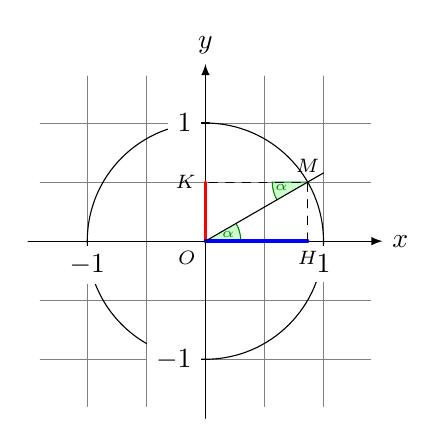
\begin{tikzpicture}[scale=1.5,cap=round]
    % Local definitions
    \def\costhirty{0.8660256}
    % Colors
    \colorlet{anglecolor}{green!50!black}
    \colorlet{sincolor}{red}
    \colorlet{tancolor}{orange!80!black}
    \colorlet{coscolor}{blue}
    % Styles
    \tikzstyle{axes}=[>=latex]
    \tikzstyle{important line}=[very thick]
    \tikzstyle{information text}=[rounded corners,fill=red!10,inner sep=1ex]
    % The graphic
    \draw[style=help lines,step=0.5cm] (-1.4,-1.4) grid (1.4,1.4);
    \draw (0,0) circle (1cm);
    \begin{scope}[style=axes]
        \draw[->] (-1.5,0) -- (1.5,0) node[right] {$x$} coordinate(x axis);
        \draw[->] (0,-1.5) -- (0,1.5) node[above] {$y$} coordinate(y axis);
        \foreach \x in {-1,1} \draw[xshift=\x cm] (0pt,1pt) -- (0pt,-1pt) node[below,fill=white] {$\x$};
        \foreach \y in {-1,1} \draw[yshift=\y cm] (1pt,0pt) -- (-1pt,0pt) node[left,fill=white] {$\y$};
    \end{scope}
    \filldraw[fill=green!20,draw=anglecolor] (0,0) -- (3mm,0pt) arc(0:30:3mm);
    \draw (15:2mm) node[anglecolor] {\tiny$\alpha$};
    \filldraw[fill=green!20,draw=anglecolor] (\costhirty,0.5) -- ++(-3mm,0pt) arc(180:210:3mm);
    \draw (30:0.9cm) node[anglecolor,left] {\tiny$\alpha$};
    \draw[style=important line,sincolor] (0,0) -- (0,0.5);
    \draw[style=important line,coscolor] (30:1cm |- x axis) -- (0,0);
    \draw[dashed] (30:1cm |- x axis) -- (30:1cm) -- (30:1cm -| y axis);
    \draw (intersection of 0,0--30:1cm and 1,0--1,1) coordinate (t);
    \draw (0,0) -- (t);
    \draw (30:1cm) node[above] {\scriptsize$M$};
    \draw (\costhirty,0) node[below] {\scriptsize$H$};
    \draw (0,0.5) node[left] {\scriptsize$K$};
    \draw (0,0) node[below left] {\scriptsize$O$};
\end{tikzpicture}
\end{center}

Les triangles $OKM$ et $OHM$ ont la même hypoténuse $[OM]$ qui est un rayon du cercle. Donc $OM = 1$.
On utilise les définitions et on a :
\[\cos(\alpha) = \frac{OH}{OM} = OH \qetq \sin(\alpha) = \frac{OK}{OM} = OH.\]
\end{Demo}

\subsection{Relations à connaître}

\begin{Prop}
    On considère un angle de mesure $\theta$. On a les relations suivantes :
    \begin{enumerate}
        \item $\cos(-\theta) = \cos(\theta)$ et $\sin(-\theta) = -\sin(\theta)$.
        \item $\cos(\pi -\theta) = -\cos(\theta)$ et $\sin(\pi-\theta) = \sin(\theta)$.
    \end{enumerate}
\end{Prop}

\begin{Demo}
    Le plus simple est d'utiliser une figure géométrique :

    \begin{center}
        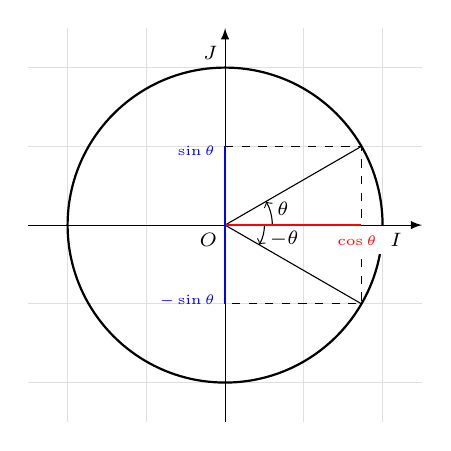
\begin{tikzpicture}
            \draw[thin, color=gray!25] (-2.5,-2.5) grid (2.5,2.5);
            \draw[thick] (0,0) circle (2cm);
            \draw[->,>=latex] (-2.5,0)--(2.5,0);
            \draw[->,>=latex] (0,-2.5)--(0,2.5);
            \coordinate (O) at (0,0);
            \coordinate (I) at (2,0);
            \coordinate (J) at (0,2);
            \coordinate (M) at (30:2cm); \draw (O) -- (M);
            \coordinate (N) at (-30:2cm); \draw (O) -- (N);
            \begin{scriptsize}
                \draw (O) node[below left]{$O$};
                \draw (I) node[below right]{$I$};
                \draw (J) node[above left]{$J$};
                \draw[->] (0.6,0) arc (0:30:0.6cm);
                \draw (20:0.6cm) node[right] {$\theta$};
                \draw[->] (0.5,0) arc (0:-30:0.5cm);
                \draw (-20:0.5cm) node[right] {$-\theta$};
            \end{scriptsize}
            \draw[dashed] (0,1) --({2*0.8660256},1) -- ({2*0.8660256},-1) -- (0,-1);
            \draw[red,thick] (0,0) -- ({2*0.8660256},0) node[below right, near end,fill=white]{\tiny $\cos\theta$};
            \draw[blue,thick] (0,0) -- (0,1) node[above left, near end]{\tiny $\sin\theta$};
            \draw[blue,thick] (0,0) -- (0,-1) node[below left, near end]{\tiny $-\sin\theta$};
        \end{tikzpicture}
        \hspace{1cm}
        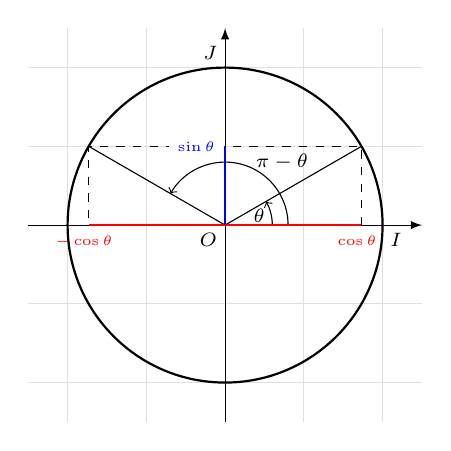
\begin{tikzpicture}
            \draw[thin, color=gray!25] (-2.5,-2.5) grid (2.5,2.5);
            \draw[thick] (0,0) circle (2cm);
            \draw[->,>=latex] (-2.5,0)--(2.5,0);
            \draw[->,>=latex] (0,-2.5)--(0,2.5);
            \coordinate (O) at (0,0);
            \coordinate (I) at (2,0);
            \coordinate (J) at (0,2);
            \coordinate (M) at (30:2cm); \draw (O) -- (M);
            \coordinate (N) at (150:2cm); \draw (O) -- (N);
            \begin{scriptsize}
                \draw (O) node[below left]{$O$};
                \draw (I) node[below right]{$I$};
                \draw (J) node[above left]{$J$};
                \draw[->] (0.6,0) arc (0:30:0.6cm);
                \draw (15:0.45cm) node {$\theta$};
                \draw[->] (0.8,0) arc (0:150:0.8cm);
                \draw (70:0.85cm) node[right] {$\pi-\theta$};
            \end{scriptsize}
            \draw[dashed] ({2*0.8660256},0) -- ({2*0.8660256},1) -- ({-2*0.8660256},1) -- ({-2*0.8660256},0);
            \draw[red,thick] (0,0) -- ({2*0.8660256},0) node[below right, near end]{\tiny $\cos\theta$};
            \draw[red,thick] (0,0) -- ({-2*0.8660256},0) node[below left, near end]{\tiny $-\cos\theta$};
            \draw[blue,thick] (0,0) -- (0,1) node[fill=white,left]{\tiny $\sin\theta$};
        \end{tikzpicture}
    \end{center}
\end{Demo}

\subsection{Quelques équations trigonométriques}
La propriété précédente nous permet alors de résoudre quelques équations où apparaissent soit le cosinus, soit le sinus.

\begin{Prop}
    Soit $a$ un nombre fixé.\par
    L'équation $\cos (t) = \cos (a)$ admet une \textbf{infinité} de solutions pouvant s'écrire sous l'une des deux formes suivantes :
    \[t = a + 2k\pi, k \in \Z \qquad \text{ou} \qquad t = -a + 2k\pi, k \in \Z\]
\end{Prop}

\begin{Exemple}
    Donner toutes les solutions de l'équation suivantes puis la mesure principale des angles qui vérifient l'équation :
    \[\cos(t) = \cos\left(\frac\pi3\right).\]
    Les solutions sont de la forme $t = \frac\pi3 + 2k\pi (k \in Z)$ ou $t = -\frac\pi3 + 2k\pi (k \in \Z)$.\par
    Par exemple, voici quelques solutions :
    \[
    \renewcommand\arraystretch{2.75}
    \begin{array}{|c|c|c|}
    \hline
        k = 0 & \frac\pi3 & -\frac\pi3\\
    \hline
        k = 1 & \frac{7\pi}{3} & \frac{5\pi}{3}\\
    \hline
        k = -1 & -\frac{5\pi}{3} & -\frac{7\pi}{3}\\
    \hline
        k = 2 & \frac{13\pi}{3} & \frac{11\pi}{3} \\
    \hline
        k = -2 & -\frac{11\pi}{3} & -\frac{13\pi}{3} \\
    \hline
    \end{array}
    \]
    $\frac \pi 3$ et $-\frac\pi3$ sont les mesures principales des angles solutions.
\end{Exemple}

\begin{Prop}
    Soit $a$ un nombre fixé.\par
    L'équation $\sin (t) = \sin (a)$ admet une \textbf{infinité} de solutions pouvant s'écrire sous l'une des deux formes suivantes :
    \[t = a + 2k\pi, k \in \Z \qquad \text{ou} \qquad t = \pi -a + 2k\pi, k \in \Z\]
\end{Prop}

\begin{Exemple}
    Donner toutes les solutions de l'équation suivantes puis la mesure principale des angles qui vérifient l'équation :
    \[\sin(t) = \sin\left(\frac\pi6\right).\]
    Les solutions sont de la forme $t = \frac\pi6 + 2k\pi (k \in Z)$ ou $t = \underbrace{\pi-\frac\pi6}_{=\frac{5\pi}{6}} + 2k\pi (k \in \Z)$.\par
    Par exemple, voici quelques solutions :
    \[
    \renewcommand\arraystretch{2.75}
    \begin{array}{|c|c|c|}
    \hline
        k = 0 & k = 1 & k = -1\\
    \hline
        \frac\pi6 & \frac{13\pi}{6} & -\frac{11\pi}{6}\\
    \hline
        \frac{5\pi}{6} & \frac{17\pi}{6} & -\frac{7\pi}{6}\\
    \hline
    \end{array}
    \]
    $\frac \pi 6$ et $\frac{5\pi}{6}$ sont les mesures principales des angles solutions.
\end{Exemple}

\end{document}
